\section{Hardwareimplementering}
Alle dele af projektets hardware er blevet analyseret og designet og derefter implementeret. Vi startede med at udregne komponenter til forstærkeren, som vi på forhånd vidste hvordan skulle opbygges. Efter beregningerne kunne forstærkeren opbygges på fumlebræt. Efter at hver del er blevet implementeret på fumlebrættet er det blevet modultestet. På denne måde er vi sikre på, at hvert delelement af projektets hardware virker som forventet. På fumlebrættet er forstærkeren, subtractoren og Sallen-Key filteret derved implementeret og modultestet enkeltvis for at se om de gav de forventede værdier. Efterfølgende blev det hele sat sammen til et kredsløb og systemet kunne derefter integrationstestes. 

\begin{figure}[h!]
	\centering
	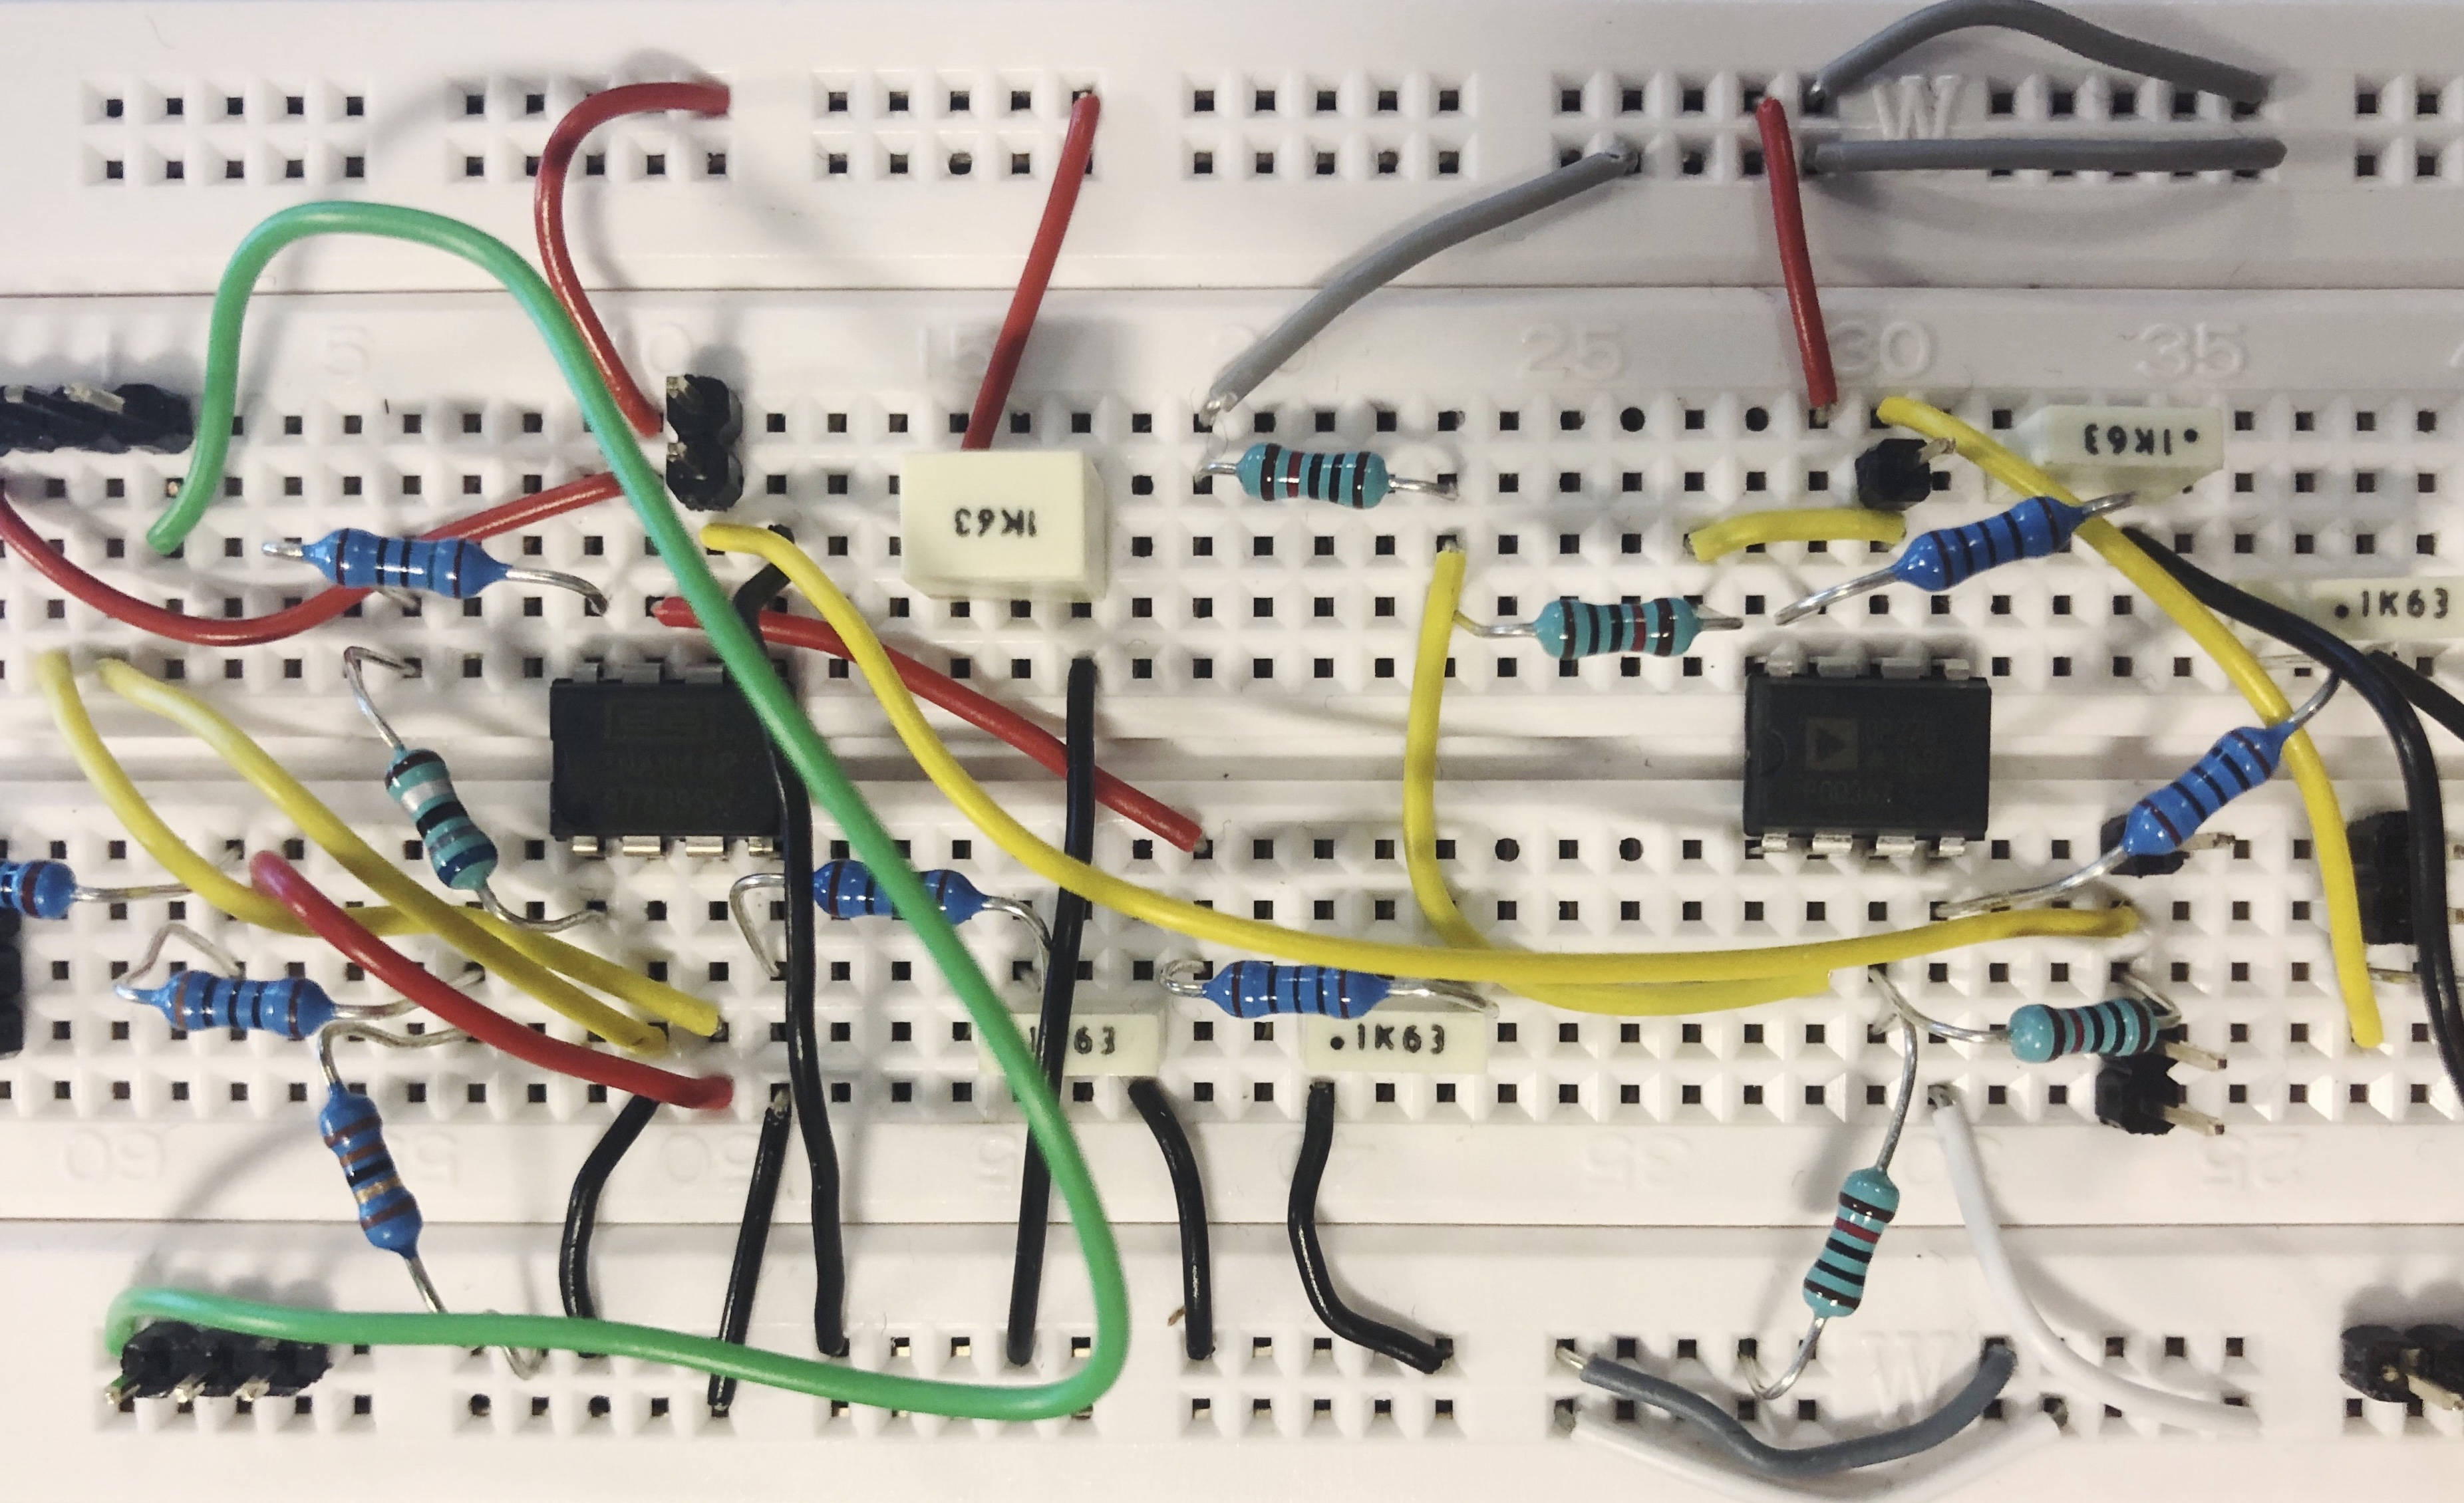
\includegraphics
	[width=0.54\linewidth]{../Rapport/Implementering_og_test/Hardware/forstaerkerogsubtractor2}
	\caption{Opbygning af forstærker(til venstre) og subtractor (til højre) på fumlebræt}
	\label{fig:forstaerkerogsubtractor1}
\end{figure}

\begin{figure}[h!]
	\centering
	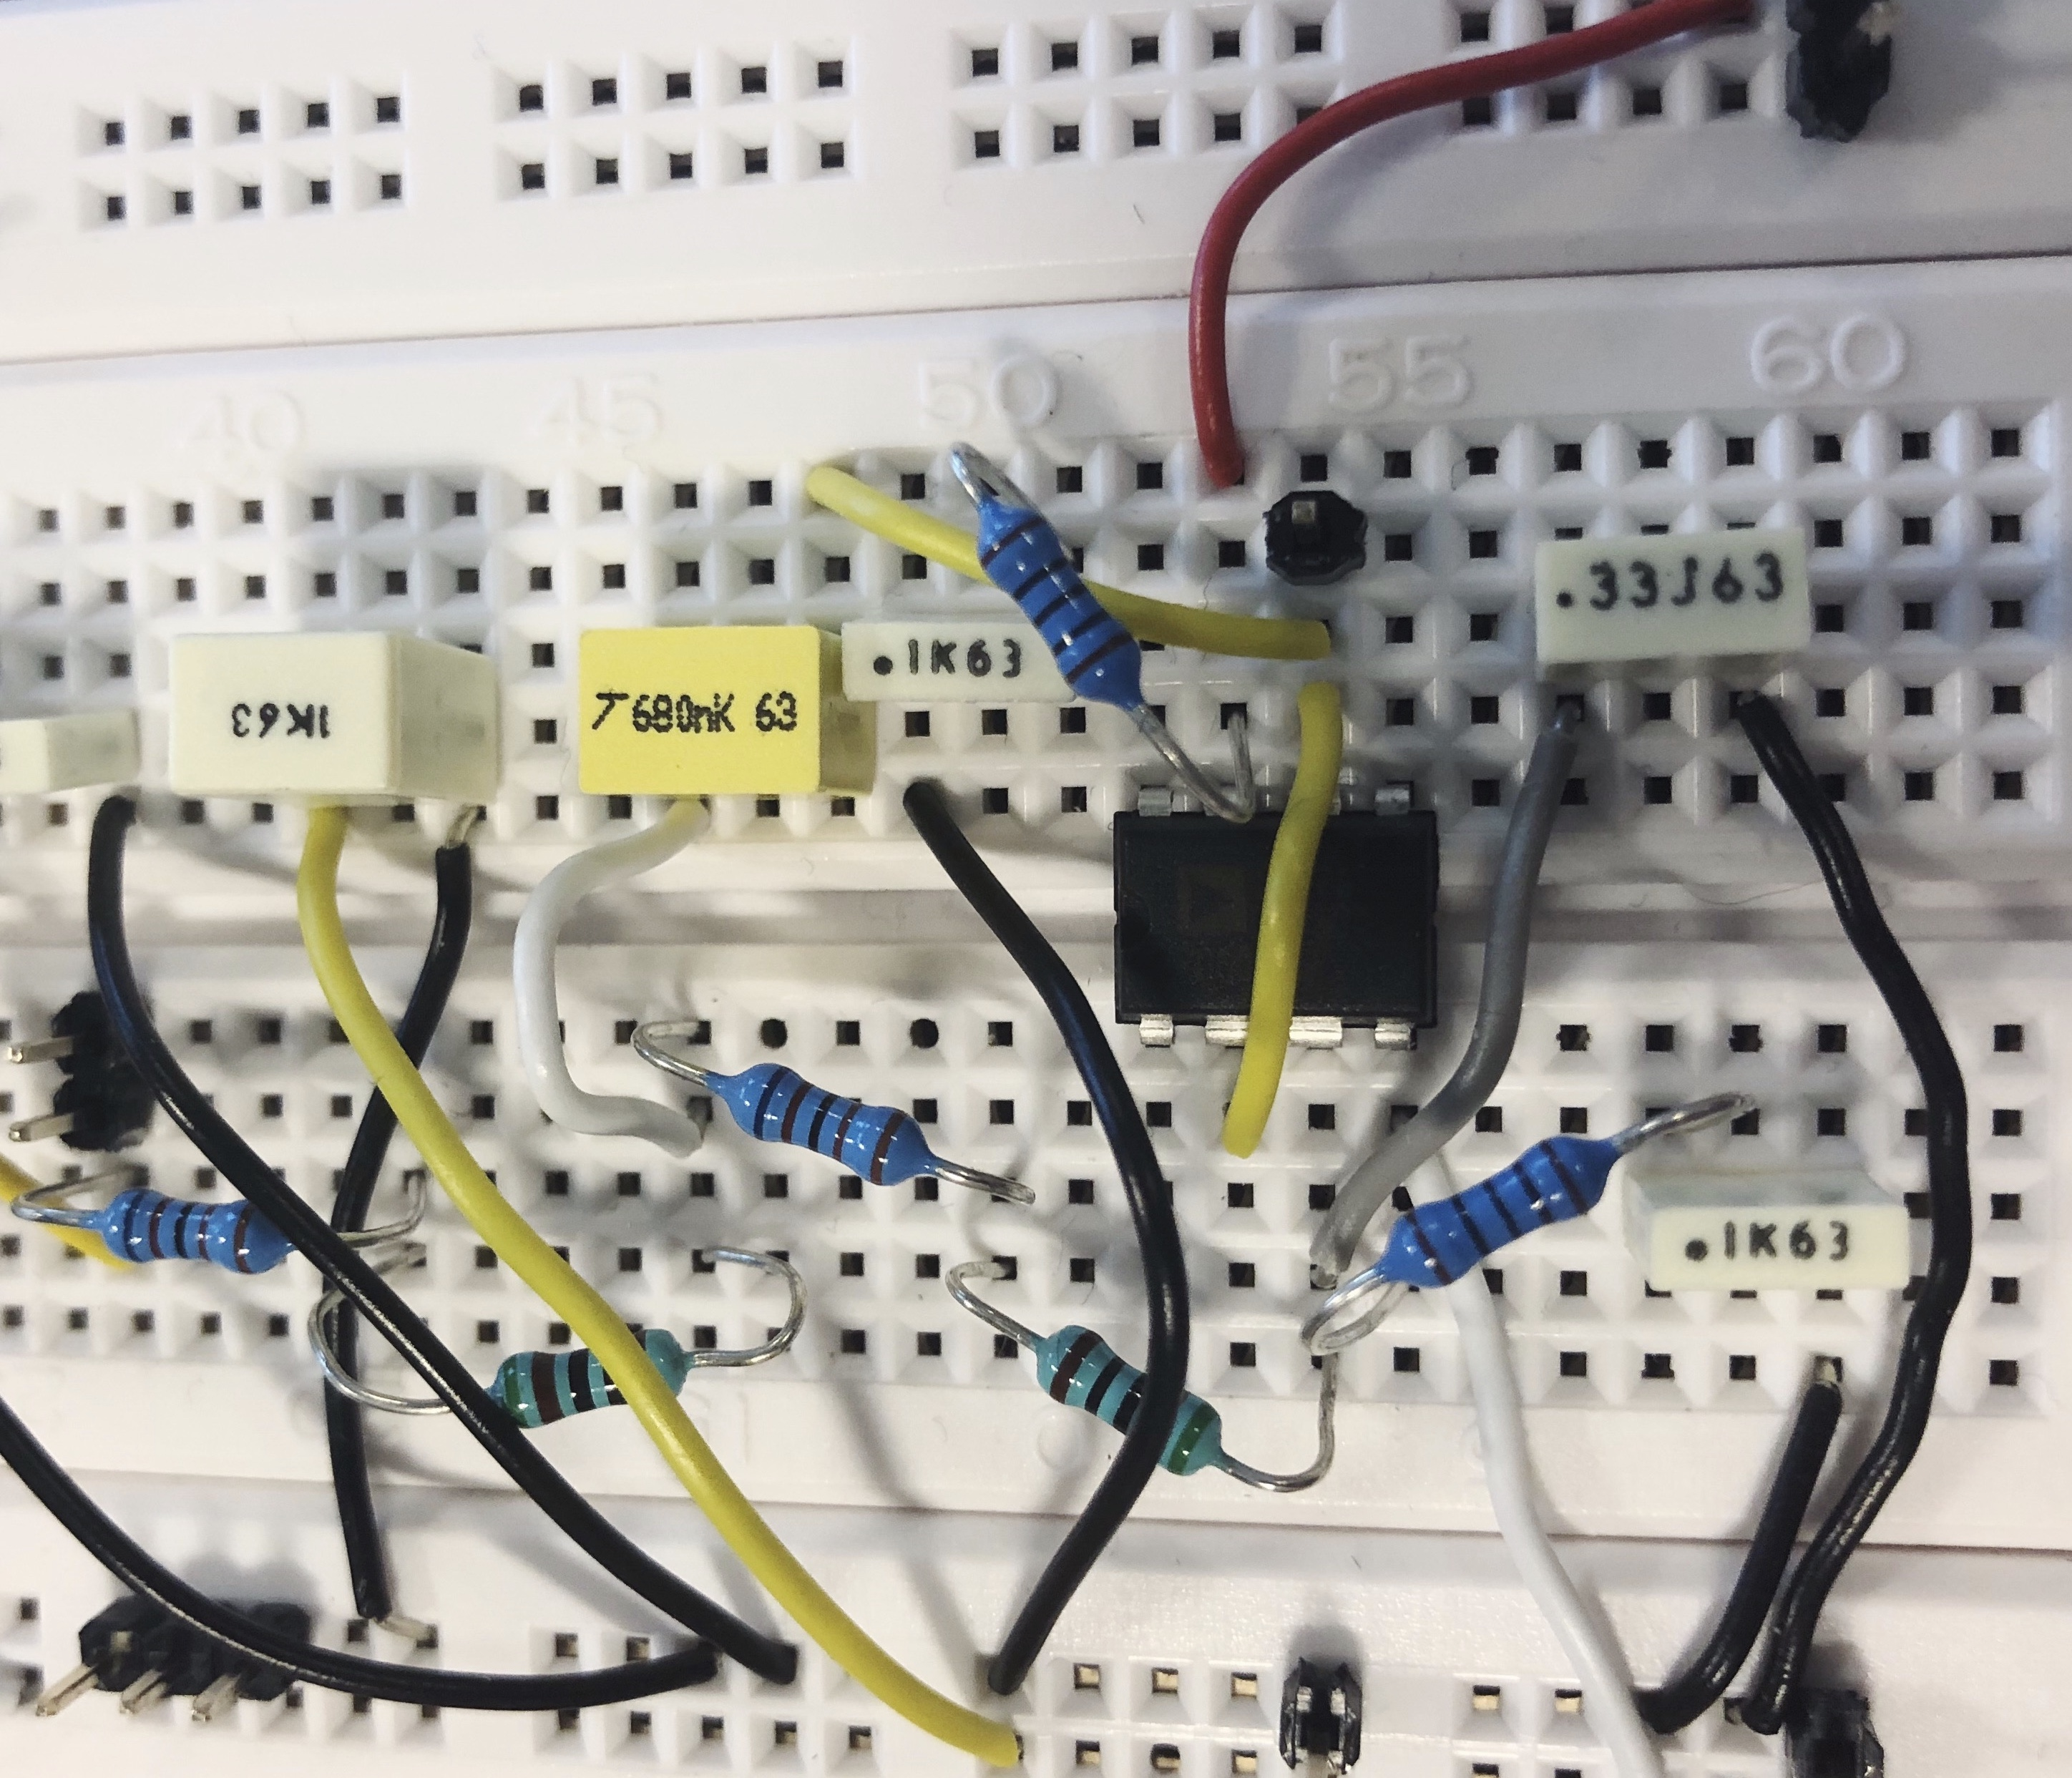
\includegraphics
	[width=0.54\linewidth]{../Rapport/Implementering_og_test/Hardware/filter2}
	\caption{Opbygning af filter på fumlebræt}
	\label{fig:filter1}
\end{figure}

Efter integrationstesten blev kredsløbet tegnet i Multisim. Det tegnede kredsløb i Multisim blev til slut overført til ultiboard, hvor de tilhørende komponenter blev placeret på printpladen. Printet blev testet og sendt til EuroCircuits. De beregnede komponenter i analyse-delen er til slut loddet på den færdige printplade og systemet blev testet en sidste gang. 

For kredsløbet i Multisim henvises til figur \vref{fig:Multisim2}. Nedenfor vises designet af printpladen i Ultiboard da det var klar til print samt printpladen, der er loddet med alle komponenter.

\begin{figure}[h!]
	\centering
	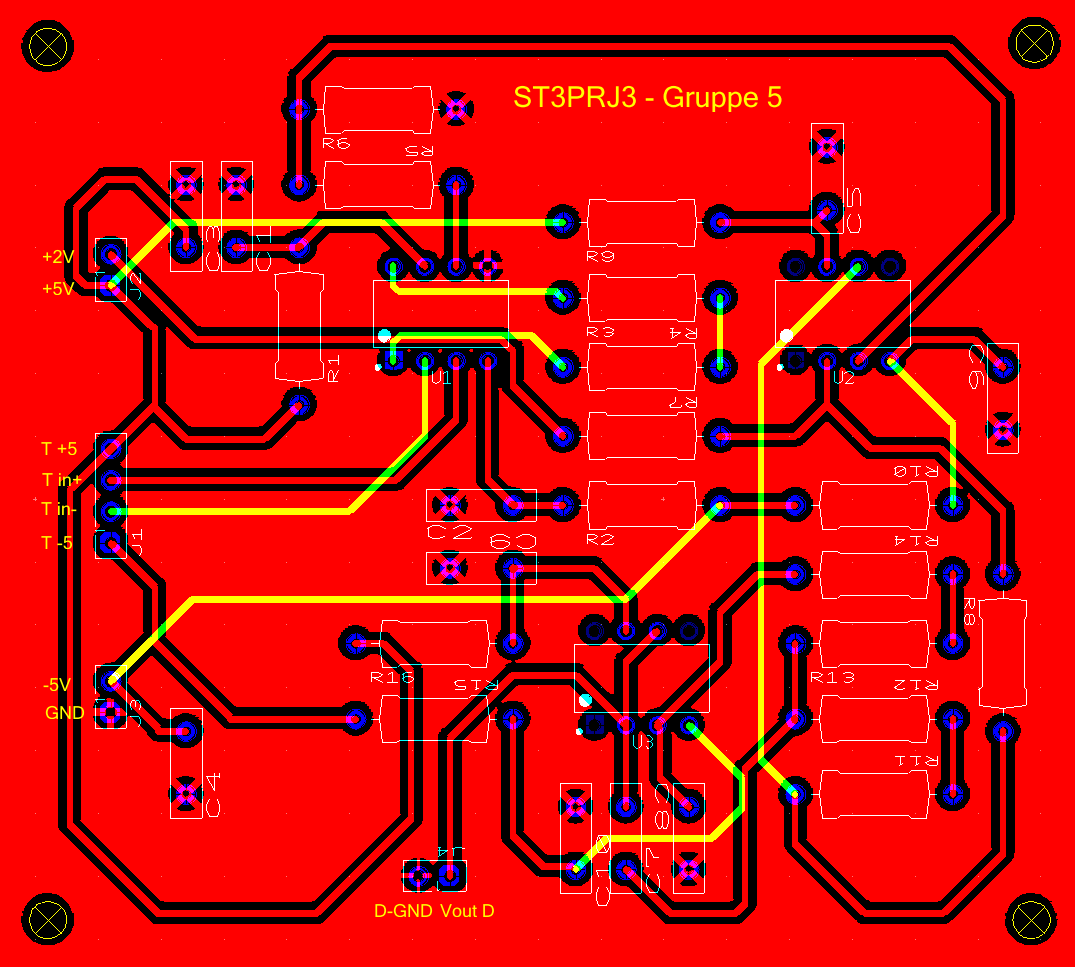
\includegraphics[width=0.5\linewidth]{../Rapport/Implementering_og_test/Hardware/Ultiboard}
	\caption{Print i Ultiboard}
	\label{fig:ultiboard1}
\end{figure}
